\documentclass[11pt]{article}

% some definitions for the title page
\newcommand{\reporttitle}{VANs and GANs}
\newcommand{\reportdescription}{Lecture notes on the Variational Encoder Networks~\cite{DBLP:journals/corr/abs-1906-02691} and the Generative Adversarial Networks~\cite{goodfellow2014generative}}

% load some definitions and default packages
%---------------------------------------------------------------------------
%	PACKAGES AND OTHER DOCUMENT CONFIGURATIONS
%---------------------------------------------------------------------------

\usepackage[twoside]{fancyhdr}
\usepackage{csquotes}

\usepackage[a4paper,hmargin=2.0cm,vmargin=1.0cm,includeheadfoot]{geometry}
% \usepackage{natbib} % for bibliography
\usepackage{biblatex}
\usepackage{tabularx,longtable,multirow,subfigure,caption}%hangcaption
\usepackage{fancyhdr} % page layout
\usepackage{url} % URLs
\usepackage[english]{babel}
\usepackage{graphicx}
\usepackage{rotating}
\usepackage{dsfont}
\usepackage{epstopdf} % automatically replace .eps with .pdf in graphics
% \usepackage{backref} % needed for citations
\usepackage{array}
\usepackage{latexsym}
\usepackage[pdftex,hypertexnames=false,colorlinks]{hyperref} % provide links in pdf (had pagebackref)
\usepackage{booktabs}
\usepackage{wrapfig}
\usepackage{caption}  % Required for \captionof
\usepackage{float} % for H option in figures
\usepackage{amssymb}
\usepackage{amsmath}
\usepackage{amsthm}
\usepackage{mathtools} % for 'dcases*' env.
\usepackage[nottoc]{tocbibind}

%%% Default fonts
\renewcommand*{\rmdefault}{bch}
\renewcommand*{\ttdefault}{cmtt}

%%% Default settings (page layout)
\setlength{\parindent}{0em}  % indentation of paragraph
\setlength{\parskip}{.3em}
\setlength{\itemsep}{0.mm}

\setlength{\headheight}{14.5pt}
\pagestyle{fancy}

\fancyfoot[ER,OL]{\thepage}%Page no. in the left on odd pages and on right on even pages

\fancyfoot[OC,EC]{\sffamily }
\renewcommand{\headrulewidth}{0.1pt}
\renewcommand{\footrulewidth}{0.1pt}
\captionsetup{margin=10pt,font=small,labelfont=bf}

% LISTINGS ammendments
\usepackage{listings}
\usepackage{color}

\definecolor{mygreen}{rgb}{0,0.6,0}
\definecolor{mygray}{rgb}{0.5,0.5,0.5}
\definecolor{mymauve}{rgb}{0.58,0,0.82}

\lstset{ 
  postbreak=\mbox{\textcolor{red}{$\hookrightarrow$}\space},
  backgroundcolor=\color{white},   % choose the background color; you must add \usepackage{color} or \usepackage{xcolor}; should come as last argument
  basicstyle=\footnotesize,        % the size of the fonts that are used for the code
  breakatwhitespace=false,         % sets if automatic breaks should only happen at whitespace
  breaklines=true,                 % sets automatic line breaking
  captionpos=b,                    % sets the caption-position to bottom
  commentstyle=\color{mygreen},    % comment style
%   deletekeywords={...},            % if you want to delete keywords from the given language
%   escapeinside={\%*}{*)},          % if you want to add LaTeX within your code
  extendedchars=true,              % lets you use non-ASCII characters; for 8-bits encodings only, does not work with UTF-8
  firstnumber=1,                % start line enumeration with line 1000
  frame=single,	                   % adds a frame around the code
  keepspaces=true,                 % keeps spaces in text, useful for keeping indentation of code (possibly needs columns=flexible)
  columns=fullflexible,
  keywordstyle=\color{blue},       % keyword style
  language=python,                 % the language of the code
  % morekeywords={*,...},            % if you want to add more keywords to the set
  numbers=left,                    % where to put the line-numbers; possible values are (none, left, right)
  numbersep=5pt,                   % how far the line-numbers are from the code
  numberstyle=\tiny\color{mygray}, % the style that is used for the line-numbers
  rulecolor=\color{black},         % if not set, the frame-color may be changed on line-breaks within not-black text (e.g. comments (green here))
  showspaces=false,                % show spaces everywhere adding particular underscores; it overrides 'showstringspaces'
  showstringspaces=false,          % underline spaces within strings only
  showtabs=false,                  % show tabs within strings adding particular underscores
  stepnumber=1,                    % the step between two line-numbers. If it's 1, each line will be numbered
  stringstyle=\color{mymauve},     % string literal style
  tabsize=2,	                   % sets default tabsize to 2 spaces
  title=\lstname% show the filename of files included with \lstinputlisting; also try caption instead of title
}

% Here, you can define your own macros. Some examples are given below.

\newcommand{\R}[0]{\mathds{R}} % real numbers
\newcommand{\Z}[0]{\mathds{Z}} % integers
\newcommand{\N}[0]{\mathds{N}} % natural numbers
\newcommand{\C}[0]{\mathds{C}} % complex numbers
\renewcommand{\vec}[1]{{\boldsymbol{{#1}}}} % vector
\newcommand{\mat}[1]{{\boldsymbol{{#1}}}} % matrix


\usepackage{pdfpages}

\bibliography{bibliography}

\begin{document}

% Include the title page
\begin{titlepage}

    \newcommand{\HRule}{\rule{\linewidth}{0.5mm}} % Defines a new command for the horizontal lines, change thickness here
    
    \center % Center everything on the page
     
    %------------------------------------------------------------------------
    %	HEADING SECTIONS
    %------------------------------------------------------------------------
    
    \textsc{\Large Department of Computing}\\[0.5cm] 
    \textsc{\large Imperial College of Science, Technology and Medicine}\\[0.5cm] 
    
    %------------------------------------------------------------------------
    %	TITLE SECTION
    %------------------------------------------------------------------------
    
    \HRule \\[0.4cm]
    { \huge \bfseries \reporttitle}\\ % Title of your document
    \HRule \\[0.4cm]

    \textit{\reportdescription}
    
    \vspace{2em}

    %------------------------------------------------------------------------
    %	AUTHOR SECTION
    %------------------------------------------------------------------------
    
    \large \emph{Author: Anton Zhitomirskiy}

    \vspace{1em}

    \global\let\newpagegood\newpage
    \global\let\newpage\relax
    
\end{titlepage}

\global\let\newpage\newpagegood

\tableofcontents

\clearpage

\section{Introduction}\label{sect:Introduction}

\subsection{Supervised Learning}\label{sect:Supervised Learning}

Supervised learning is a process which attempts to learn patterns amongst data to predict a label $y$ given an imput $x$, i.e. learn a function to map $x\rightarrow y$. For this to work, supervised learning uses labelled data inputs $(x,y)$ to train its parameters.

\begin{equation}\label{eq:supervised-underlying-data-distribution}
    \text{Data: } (x_1, y_1), \dots , (x_N, y_N) \sim p_{data}(x,y)
\end{equation}

\subsection{Unsupervised Learning}\label{sect:Unsupervised Learning}

However, most of the data we have available isn't well-formed pairs of labelled data. It just an anonymous data point. Thus, the task is now to inferr a function that describes the hidden structure of unlabelled data.

\begin{equation}\label{eq:unsupervised-underlying-data-distribution}
    \text{Data: } x_1, \dots , x_N \sim p_{data}(x) \quad \text{no supervision signal}
\end{equation}

\subsubsection{Probability Distribution/Density Estimation}\label{sect:Probability Distribution/Density Estimation}

Assume the data is sampled form an underlying data distribution (Equation~\ref{eq:unsupervised-underlying-data-distribution}) with a given probability density $p_{data}(x)$. The goal is to learn a distribution or \textbf{probabilistic model} where $\theta$ is the collection of learnable parameters.

\begin{equation}
    p_\theta(x)\approx p_{data}(x), \quad \text{with data } x_1, \dots, x_N
\end{equation}

\subsection{Generative \textbf{Latent} Variable Models}\label{sect:Generative Latent Variable Models}

Design $p_\theta(x)$ as a generative latent variable model (LVM). The idea is to describe the sampling of the oservation $x$ as a generative process where we first sample the latent variable $z$ and then generate $x$ condition on $z$.

\begin{gather}
    z \approx p_\theta(z), \quad x \approx p_\theta(x|z) \\
    \Rightarrow p_\theta(x) = \int p_\theta(x|z)p_\theta(z)dz \\
    \nonumber z: \text{latent variable (unobserved)} \quad x: \text{observed variable}
\end{gather}

Examples:

\begin{itemize}
    \item \begin{itemize}
              \item $z$: digit label, writing style, \dots
              \item $x$: hand-written digit
          \end{itemize}
    \item \begin{itemize}
              \item $z$: scene, viewing angle, lighting condition, \dots
              \item $x$: tet photo image
          \end{itemize}
    \item \begin{itemize}
              \item $z$: semantic, sentiment meaning, \dots
              \item $x$: generated text
          \end{itemize}
\end{itemize}

\subsection{Dimensionality Reduction}\label{sect:Dimensionality Reduction}

The goal is to represent the observed data points with lower dimesnional features. Given high-dimensional raw data, it is often sparse, perhaps lying ona  low-dimensional mainfold.

\subsubsection{Principal Componenet Analysis (PCA)}\label{sect:Principal Componenet Analysis (PCA)}

Given input data, PCA find the principal components to explain the variability in data as orthogonal directions that capture most of the variance in the data. The principal components are generated by magnitude, i.e. direction of gratest variability followed by the next orhogonal (uncorrelated) direction of greatest variability and so on.

In practice, we look at the first k principal components and then project the data points to the subspace span by those key princiapl componenets. Dimensionality reduction is achieved by projecting the data on the top $K < d$ princiapl components ($x\in \R^d$).

\subsubsection{Probabilistic PCA}\label{sect:Probabilistic PCA}

We can generalice PCA to a probabilistic version of it, which is still a Latent Variable Model as before.

\begin{gather}
    p(z) = \mathcal{N}(z; 0; I), \quad z \in \R^K, \quad K < d \\
    p_\theta(x|z) = \mathcal{N}(x;Wz, \theta^2 I), \quad x \in \R^d \\
    \nonumber \text{Parameters to optimize}: \theta = W \in \R^{d \times K}
\end{gather}

Probabilistic PCA again assumes the observed data $x$ is generated conditionally on a latent variable $z$. Here, the prior distribution of $x$ is a standard Gaussian, and the conditional generation process is linear.

By training the probPCA with maximum likelihood, one can show that the $W$ matrix contains the otp $K$ princiapl components, which are the top K eigenvectors of the data covariance matrix.

\subsubsection{Auto-encoders}\label{sect:Auto-encoders}

\begin{figure}[H]
    \centering
    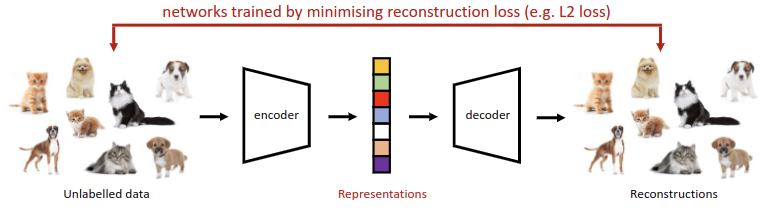
\includegraphics[width=\linewidth]{figures/auto-encoder.png}
    \caption{Encoder network extracts data representations (often with lower dimensionality) and Decoder network to reconstruct data given the representations}\label{fig:auto-encoder-1}
\end{figure}

The dimensionality is lower than the input becuase othewrise the networks can simply learn identity mappings to copy froward whatever is seen.

\subsection{Clustering}\label{sect:Clustering}

Clustering discovers group structures in unlabelled datapoints. It does so by grouping datapoints into several clusters, where datapoints in the same cluster are similar, and otherwise dissimilar.

\subsubsection{Gaussian mixture model (GMM)}\label{sect:Gaussian mixture model (GMM)}

\begin{gather}
    p_\theta(z)=Categorical(\pi), \\
    \pi = (\pi_1, \dots, \pi_k), \pi_i = p_\theta(z=1), \quad \sum^K_{i=1}\pi_i = 1 \\
    p_\theta(x|z) = \mathcal{N}(x;\mu_z; \Sigma_z) \\
    \nonumber z \in \{1, \dots K\}: \text{index of the Gaussian component} \\
    \nonumber \mu_z: \text{mean of the $i^{th}$ Gaussian component if $z=i$} \\
    \nonumber \Sigma_z: \text{Covariance matrix of the $i^{th}$ Gaussian component if $z=i$}
\end{gather}

Clustering can be done by fititng a GMM model to the data.

We can optimize the Gaussian component parmaeters and the categorical distribution on $z$ by maximum likelihood.

\subsection{Representation learning}\label{sect:Representation learning}

Both dimensionality reduction and clustering can be viewed as representation learning. The hope is for these models useful for downstream tasks.

\begin{figure}[H]
    \centering
    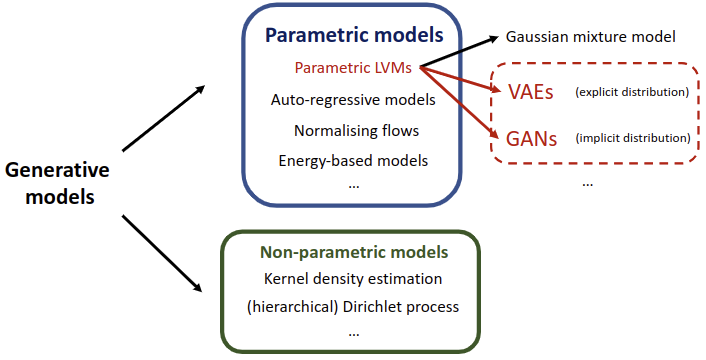
\includegraphics[width=.7\linewidth]{figures/taxonomy.png}
    \caption{}\label{fig:taxonomy}
\end{figure}

\section{Variational AutoEncoder basics}\label{sect:Variational AutoEncoder basics}

We first begin by discussing the information that is available to us:

\begin{equation}
    \underbrace{p(\theta|x)}_\text{posterior} = \frac{\overbrace{p(x|\theta)}^\text{likelihood} \cdot \overbrace{p(\theta)}^\text{prior}}{\underbrace{p(x)}_\text{evidence}}
\end{equation}

The goal is to approximate the $p_\theta(x)$ function that is learnt to closely mimic the goal $p_{data}(x)$ probability distirbution. To achieve this, we first need to consider a criterai to measure the closesness of two probability distirbutions. Then we can optimize it to make the model distribution close to the data distribution.

\subsection{Divergence minimisation}\label{sect:Divergence minimisation}

\begin{figure}[H]
    \centering
    \fbox{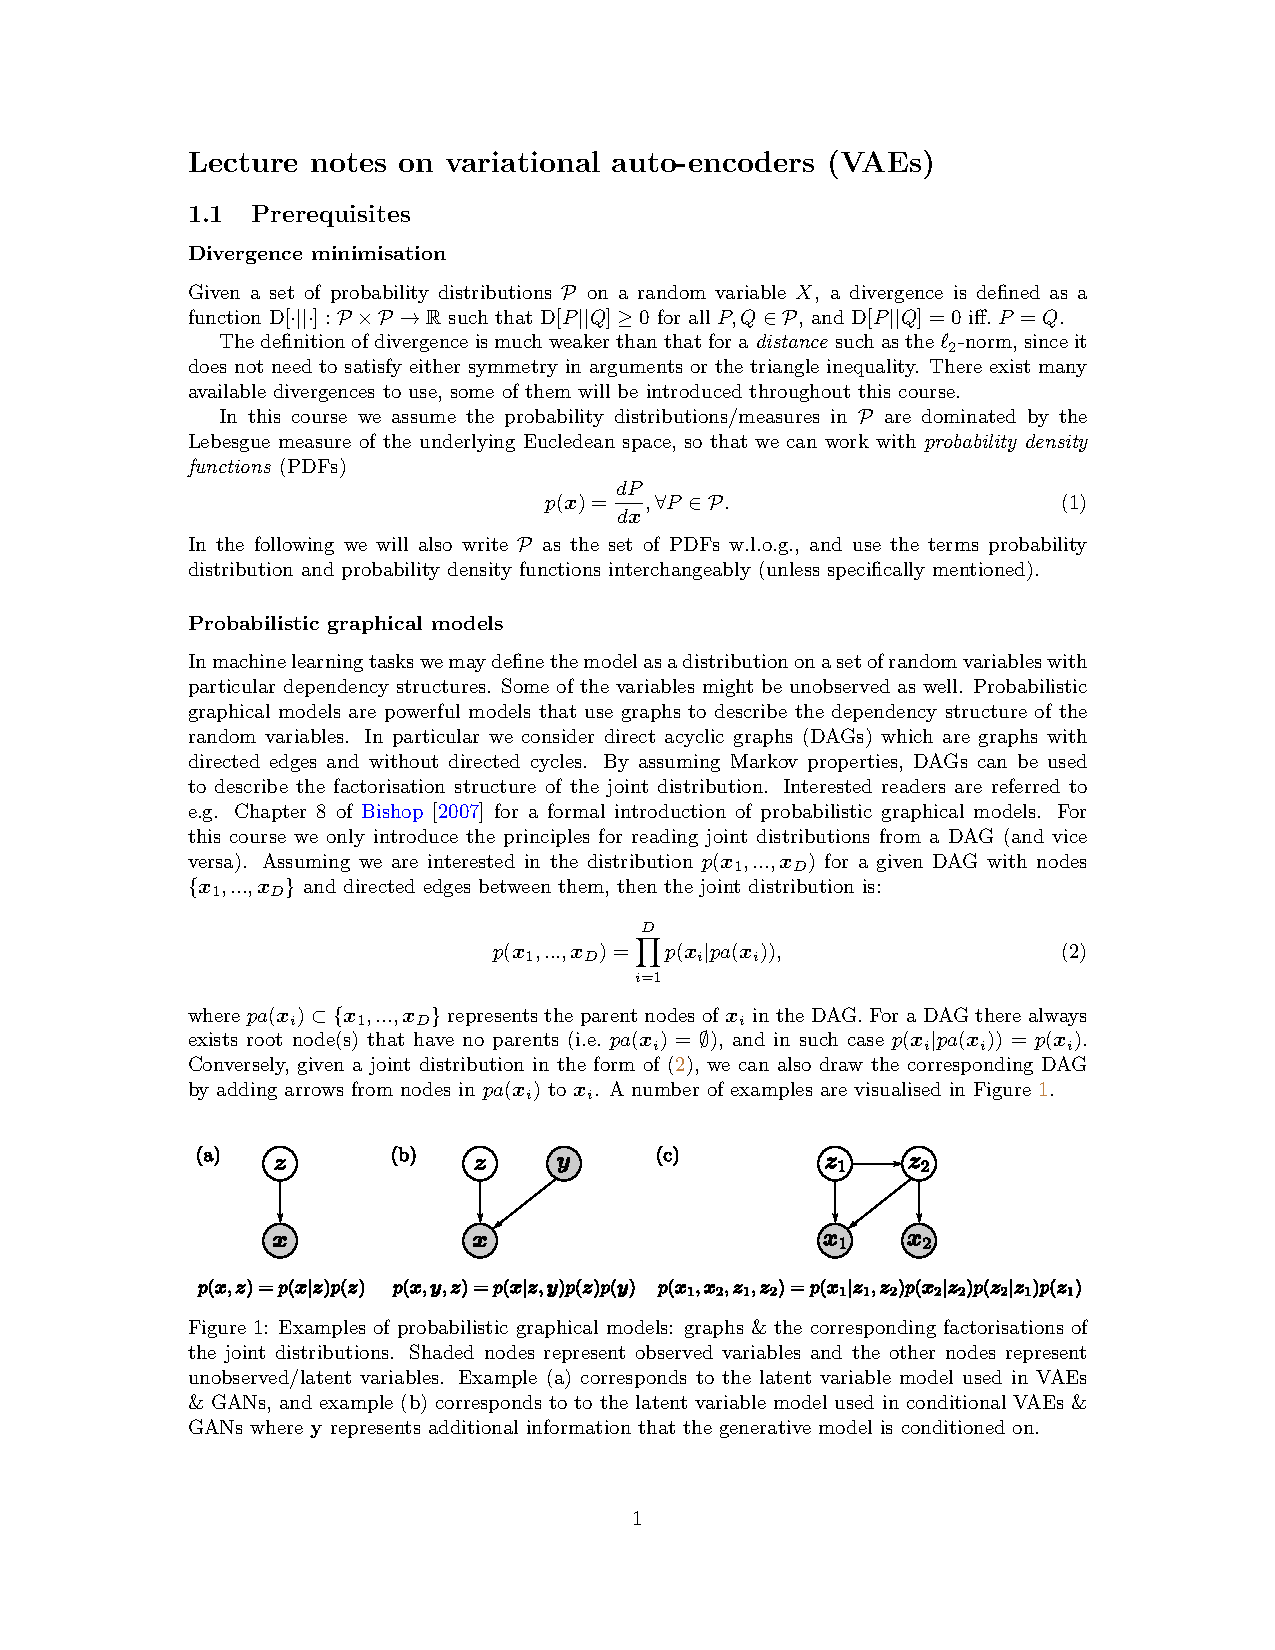
\includegraphics[page=1, trim=2.7cm 18cm 2.7cm 4.5cm, clip=true, width=\linewidth]{N08_VAE.pdf}}
\end{figure}

We can then find the best parameter settings $\theta^*$ that corresponds to the probablistic model which minimises the model distribution's divergence to the data distribution.

\begin{gather}
    \theta^* = \arg \min D[p_{data}(x) || p_\theta(x)]
\end{gather}

\subsection{Kullback-Leibler (KL) divergence}\label{sect:Kullback-Leibler (KL) divergence}

\begin{figure}[H]
    \centering
    \fbox{\includegraphics[page=2, trim=2.7cm 3.1cm 2.7cm 21cm, clip=true, width=\linewidth]{N08_VAE.pdf}}
    \caption*{Equivalently, $\text{KL}[p||q]=\mathbb E_{p(\vec x)} \big[ \log \frac{p(\vec x)}{q (\vec x)}\big]$}
\end{figure}

\begin{figure}[H]
    \centering
    \fbox{\includegraphics[page=3, trim=2.7cm 20.3cm 2.7cm 2.5cm, clip=true, width=\linewidth]{N08_VAE.pdf}}
    \caption*{
        \centering
    Note, that here $-\log x \equiv \log \frac 1 x$

    We also use Jensen's inequality~(Appendix \ref{sect:Jensen's inequality})

    $ ^1$techincally speaking $p(\vec x) = q(\vec x)$ almost everywhere.
    
    And since probability densities sum to \href{https://edstem.org/us/courses/46843/discussion/4289527}{one} then we have $-\log 1 = 0$.
    }
\end{figure}

\subsection{Maximum Likelihood Estimation}\label{sect:Maximum Likelihood Estimation}

\begin{figure}[H]
    \centering
    \fbox{\includegraphics[page=3, trim=2.7cm 11.1cm 2.7cm 8.2cm, clip=true, width=\linewidth]{N08_VAE.pdf}}
\end{figure}

The equation at (5 or 6) above, requires us to write down the likelihood of $\theta$ or, in other words, the marginal distribution of X. This means that we need to calculate the integral over the join distribution over the latent variable $z$. The conditional distirbution of $p(x|z)$ is often defined by a neural network. In this case, we cannot compute the integral because it would mean computing the network output of $z$ given all possible values of $x$. This is intractible. Since the marginal distribution is intractible then so is the Maximum Liklihood Estimation.

\subsection{Optimising a variational lower-bound}\label{sect:Optimising a variational lower-bound}

Therefore we opitimize the variational lower-bound of the maximum likelihood objective function instead. We create a lower bound to the log marginal distribution for every input x, and then the expectation of this lower bound will become the lower bound of the maximum likelihood objective.

\begin{figure}[H]
    \centering
    \fbox{\includegraphics[page=3, trim=2.7cm 3.6cm 2.7cm 18cm, clip=true, width=\linewidth]{N08_VAE.pdf}}
\end{figure}

\begin{figure}[H]
    \centering
    \fbox{\includegraphics[page=4, trim=2.7cm 19.9cm 2.7cm 2.5cm, clip=true, width=\linewidth]{N08_VAE.pdf}}
    \caption*{Here, $\mathcal L (\vec x, q, \vec \theta)$ refers to the variational lower bound. This is the quantity that variational inference aims to maximize during the optimization process.}
\end{figure}

\begin{figure}[H]
    \centering
    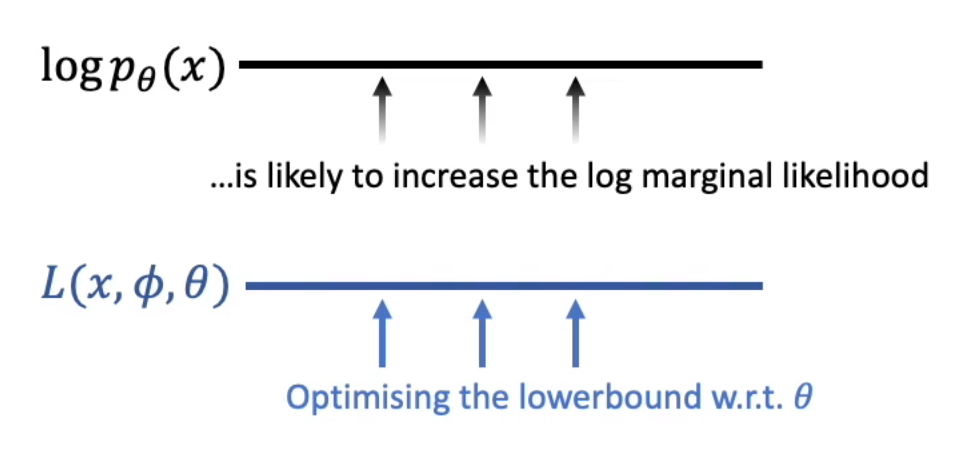
\includegraphics[width=.6\linewidth]{figures/variational-a-e.png}
    \caption{The relationship between the log marginal likelihood and the variational lower bound. }
\end{figure}

By maximising the lower bound to the log marginal distribution the marginal log liklihood itself is also likely to incrase since it is always greater than or equal to the lower bound.

\subsubsection{Alternative Approach}

\begin{figure}[H]
    \centering
    \fbox{\includegraphics[page=4, trim=2.7cm 13cm 2.7cm 8cm, clip=true, width=\linewidth]{N08_VAE.pdf}}
\end{figure}

\begin{figure}[H]
    \centering
    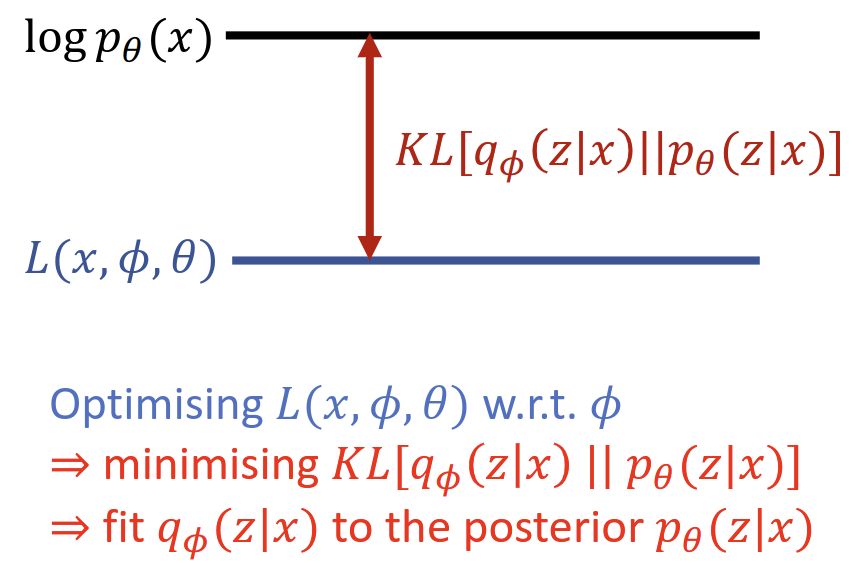
\includegraphics[width=.6\linewidth]{figures/variational-a-e-alt.png}
    \caption{The alternative relationship between the log marginal likelihood and the variational lower bound}
\end{figure}

This derrivation tells us that the gap between the marignal log likelihood and the variational lower bound is the KL divergence between the Q distribution and the example distribution.

Previously, we said that optimizing the variational lower bound w.r.t to $\theta$, is likely to optimize the marignal log likelihood. However, it doesn't happen always; it depends on the gap. 

To reduce the bias of optimizing the varaitional lower bound, we would like it to be as tight as posisble. Therefore we also optimize the variatonal lower bound w.r.t q parameters $\phi$. Since the log marginal is a constant w.r.t $\phi$ it is also equivalent to minimising the KL divergence from q to the exact posterior\footnote{Posterior probability is the probability of the parameters $\theta$ given the evidence $X$, denoted $p(\theta|X)$. This is contrary to likelihood function, which is the probability of the evidence given parameters $p(X|\theta)$}. This will fit the distribution to the approximation of the example posterior.

\subsection{Variational auto-encoders}\label{sect:Variational auto-encoders}

So far we have the following objectives:

\begin{gather}
    \theta^*, \phi^* = \arg \max L(\phi, \theta) \\
    L(\phi, \theta) := E_{p_{data}(x)}[E_{p_\phi(z|x)}[\log p_\theta(x|z)] - KL[q_\phi(z|x)||p(z)]]
\end{gather}

\begin{figure}[H]
    \centering
    \fbox{\includegraphics[page=4, trim=2.7cm 5.7cm 2.7cm 16cm, clip=true, width=\linewidth]{N08_VAE.pdf}}
\end{figure}

Auto-encoder refers to the encode-decode procedure using the q and p distribution respectively. Variational means that both both p and q are trained using the variational lower bound. 

In equation 12, similar to the generative model p, we can parameterise q with neural networks; with factorized gaussian distribution, with mean and variance of z parameterised by the neural network transform of x. In the RHS of the equation, we can parameterise the logarithm by the neural networks to ensure that the variance is non-negative.

Since the prior on z is also gaussian we can derrive an analytic form for the KL reguliser. The proof remains in the appendix at Section~\ref{sect:Analytic KL between factorised Gaussians}

\begin{figure}[H]
    \centering
    \fbox{\includegraphics[page=4, trim=2.7cm 2.9cm 2.7cm 23cm, clip=true, width=\linewidth]{N08_VAE.pdf}}
\end{figure}

\subsubsection{Reparameterisation trick}

In the VAE optimisation objective: $L(\phi, \theta) := E_{p_{data}(x)}[\underline{E_{p_\phi(z|x)}[\log p_\theta(x|z)]} - KL[q_\phi(z|x)||p(z)]]$ the underlined term is expensive to calculate. This loglikelihood term is intractible, it requires computing the expectation under the q distribution. It is still expensive to pass every z through the generative network. 

\subsubsection{Monte-carlo estimation}

We can therefore use Monte-carlo estimation to help. We can approximate the expected log likelihood return with the log-likelihood return evaluated on a single sample from the q distribution. This way we can differntiate the right-hand side of the expression with respect to $\theta$ to obtain the graident for learning $\theta$.

\begin{figure}[H]
    \centering
    \fbox{\includegraphics[page=5, trim=2.7cm 9.6cm 2.7cm 14.5cm, clip=true, width=\linewidth]{N08_VAE.pdf}}
\end{figure}

However, it is unclear how to learn the variational parameter $\phi$. We can similarly reparameterise the term

\begin{equation}
    E_{q_\phi(z|x)}[\log p_\theta(x|z)] \approx \log p_\theta(x|z), \quad z \sim q_\phi(z|x)
\end{equation}

\begin{figure}[H]
    \centering
    \fbox{\includegraphics[page=5, trim=2.7cm 7cm 2.7cm 18cm, clip=true, width=\linewidth]{N08_VAE.pdf}}
\end{figure}

\subsubsection{Reparameterisation trick}\label{sect:Reparameterisation trick}

\begin{figure}[H]
    \centering
    \fbox{\includegraphics[page=5, trim=2.7cm 3.1cm 2.7cm 21.8cm, clip=true, width=\linewidth]{N08_VAE.pdf}}
\end{figure}

\begin{figure}[H]
    \centering
    \fbox{\includegraphics[page=6, trim=2.7cm 16.9cm 2.7cm 2.5cm, clip=true, width=\linewidth]{N08_VAE.pdf}}
\end{figure}

\subsubsection{Conclusion}

\begin{figure}[H]
    \centering
    \fbox{\includegraphics[page=28, trim=2cm 2.2cm 2.8cm 5.1cm, clip=true, width=\linewidth]{L07-10_generative_models.pdf}}
\end{figure}

\begin{itemize}
    \item The first term in the variational lower bound corresponds to the reconstruction error of the auto-encoding procedure with a noteble difference, that the encoder injects a noise variable $\epsilon$ into the encoding $z$.
    \item On the figure, we see that there will be a deterministic auto-encoder if the variance of the Q distribution is 0
    \item This variance collapse is prevented by the extra KL regularisation term that is not the usual auto-encoder objective. 
    \item The auto-encoder will be stochastic after learning.
    \item The idea of the reguliser, is to make the Q distribution closer to the prior. So after learning, the stochastic encoding of the observed data will have a high probability on the prior.
\end{itemize}

\subsection{Generating data from the VAE}

Once trained sample new images from the model with 

\begin{gather}
    z \sim p(z), \quad x \sim p(x|z)
\end{gather}

Often we define z as a multivariate latent variable. The hope is after learning, different dimensions of z will encode different information of the observed data. Therefore, by varying values in different dimensions in the latent variable this \textbf{disentangles} representation.

\subsubsection{Pseudo-code}

\begin{figure}[H]
    \centering
    \fbox{\includegraphics[page=30, trim=2cm 2.25cm 2.8cm 6.5cm, clip=true, width=\linewidth]{L07-10_generative_models.pdf}}
\end{figure}

\section{GAN}

Similarly, we are trying to approximate a model $p_\theta(x) \approx p_{data}(x)$. We achieve this by tring to minimise the divergence between the model and the data, by selecting parameters in $\vec \theta$ which minimise the divergence:

\begin{equation}
    \theta^* = \arg_\theta \min D[p_{data}(x) || p_\theta(x)]
\end{equation}

\subsection{Architecture}

\begin{figure}[H]
    \centering
    \fbox{\includegraphics[page=34, trim=2cm 1cm 2.8cm 4.5cm, clip=true, width=.8\linewidth]{L07-10_generative_models.pdf}}
\end{figure}

% Assume we have drawn samples from the data distribution. Using the deep generative model, we can draw samples from the model by sampling a latent variable prior $z$ and label it as a fake image. We then build a discriminator network which generates a binary value, real or fake; a Binary Classification task (Appendix~\ref{app:gan:Binary Classification}). The objective is summarised below:

% \begin{equation}
%     \min_\theta \max_\phi L(\theta,\phi) := \mathbb E_{p_{data}(x)}[\log D_\phi(x)]+ \mathbb E_{p_{\theta}(x)}[\log(1-D_\phi(x))]
% \end{equation}

% \subsubsection{Original GAN formulation as binary classification}\label{app:gan:Original GAN formulation as binary classification}
\subsubsection{Two-player game objective}

\begin{figure}[H]
    \centering
    \fbox{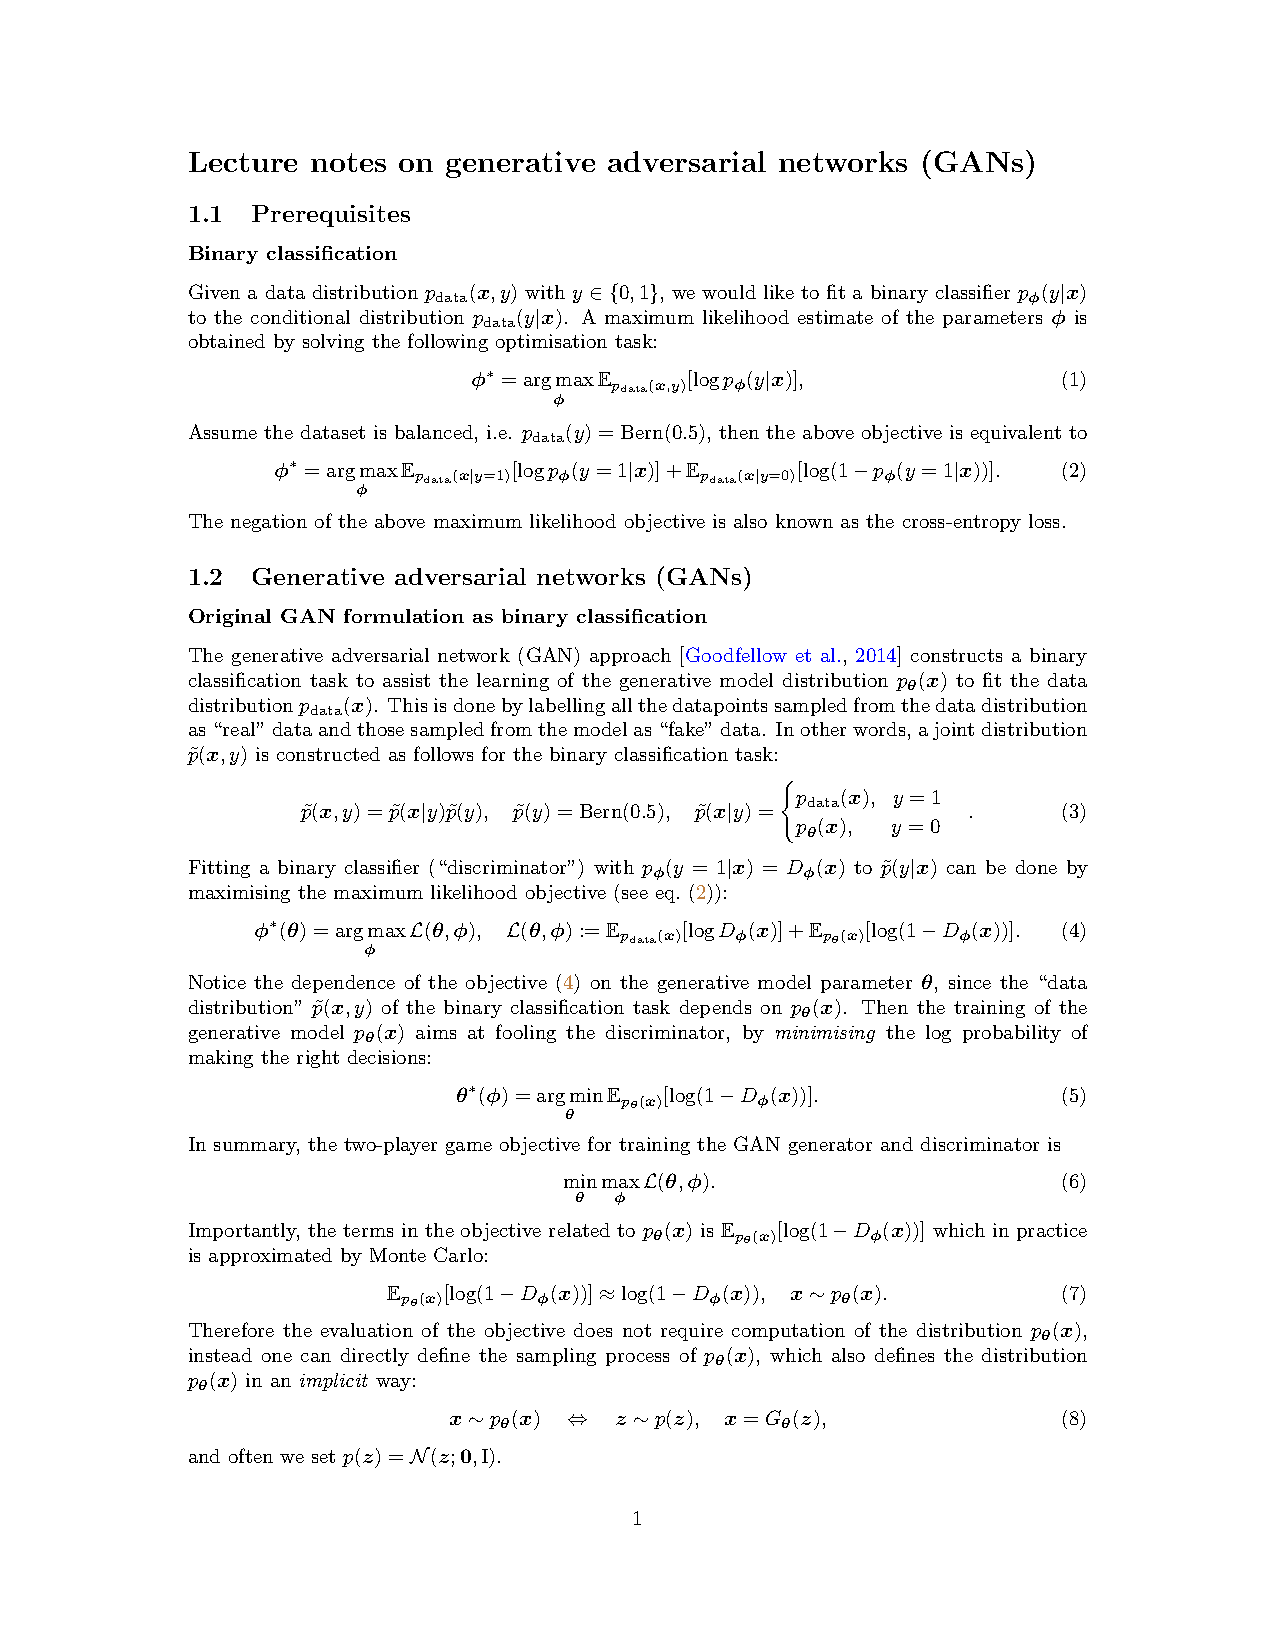
\includegraphics[page=1, trim=2.7cm 11.5cm 2.7cm 10.8cm, clip=true, width=\linewidth]{N09_GAN.pdf}}
    \caption*{We have also that $D_\phi(x):=P(x\ is\ real) \wedge 1 - D_\phi(x)=P(x\ is\ fake)$}
\end{figure}

With a fixed $\theta$: training $D_\phi$ as the classifier of the binary classification task with maximum likelihood (i.e. negative cross entropy):

\begin{gather}
    y = 1\ if\ x\sim p_{data}(x), \quad else\quad y=0\ if\ x \sim p_\theta(x)
\end{gather}

With fixed $\phi$: training $G_\theta$ to minimize the log-probability of $x \sum p_\theta(x)$ being classified as ``fake data'' by $D_\phi$.

\begin{figure}[H]
    \centering
    \fbox{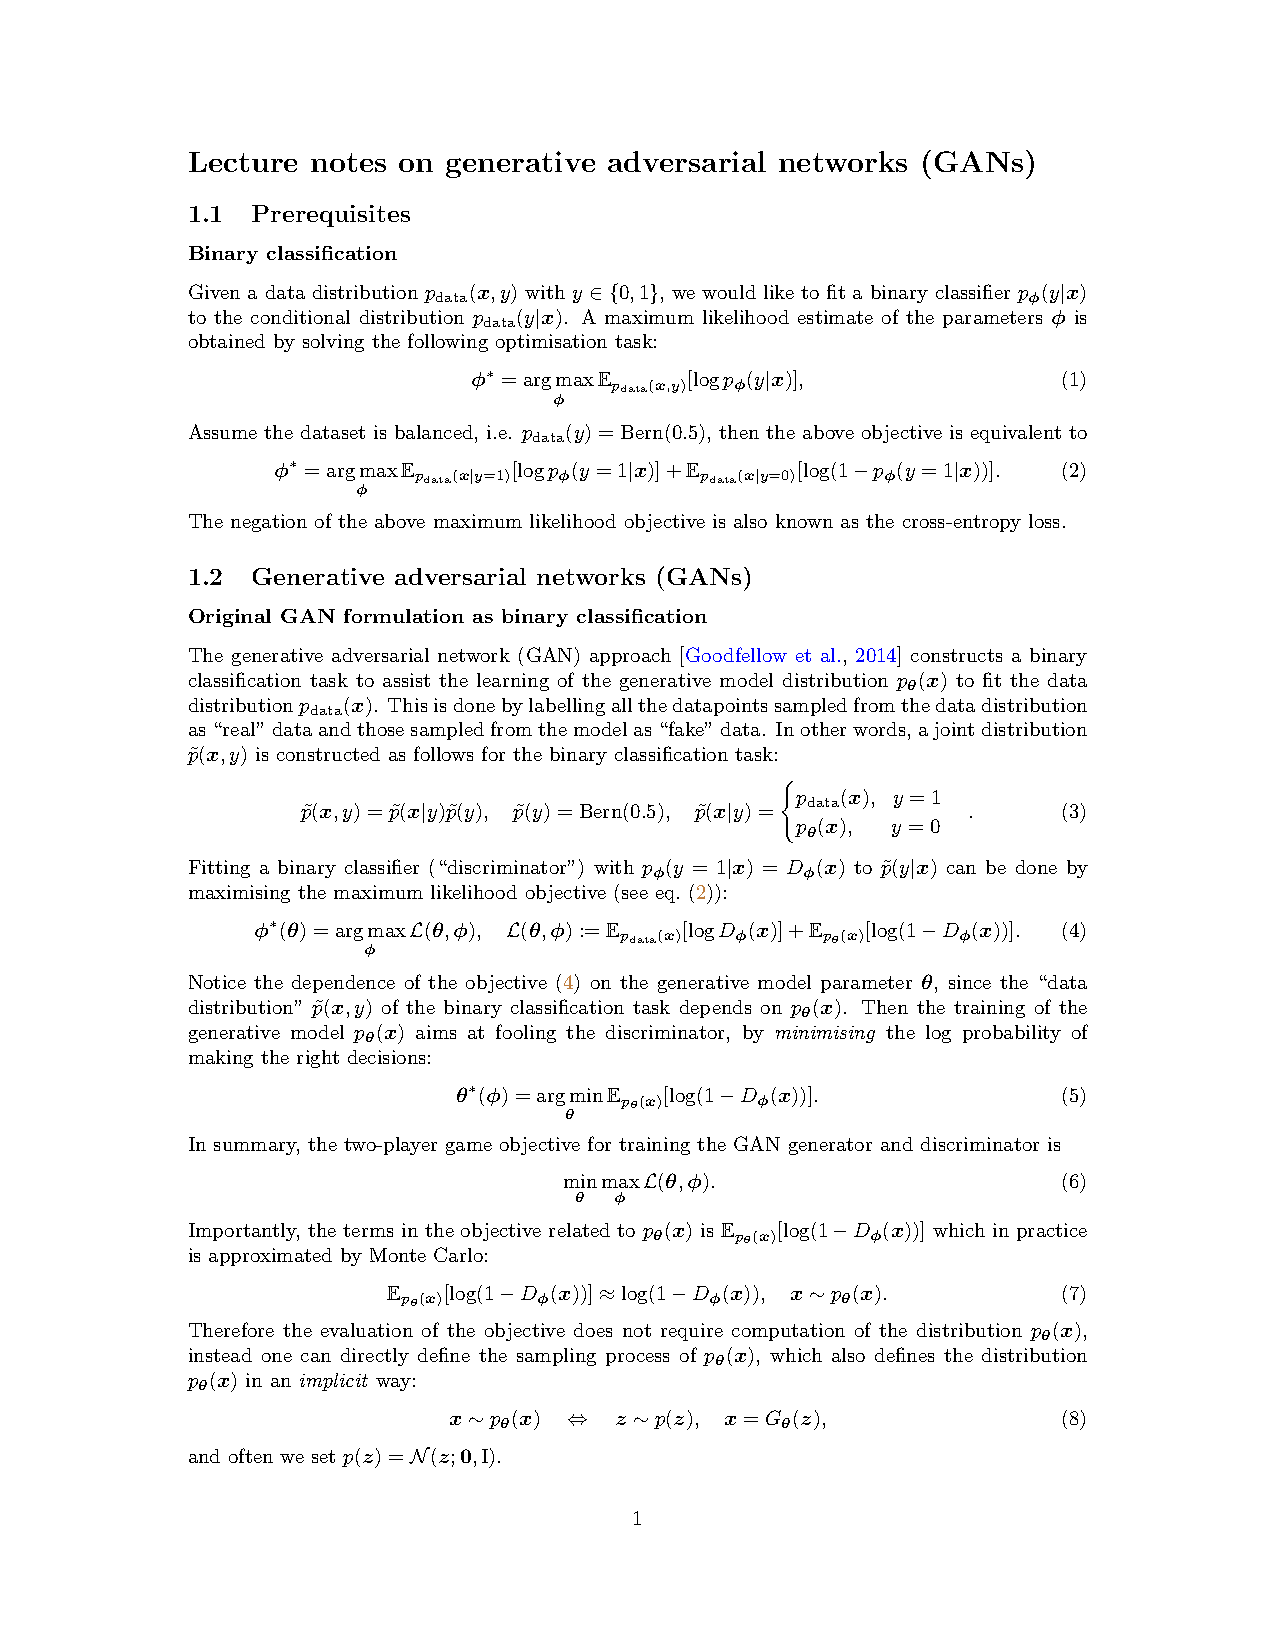
\includegraphics[page=1, trim=2.7cm 8.8cm 2.7cm 16.3cm, clip=true, width=\linewidth]{N09_GAN.pdf}}
\end{figure}
 
\subsection{Solving the two-player game objective}

\begin{figure}[H]
    \centering
    \fbox{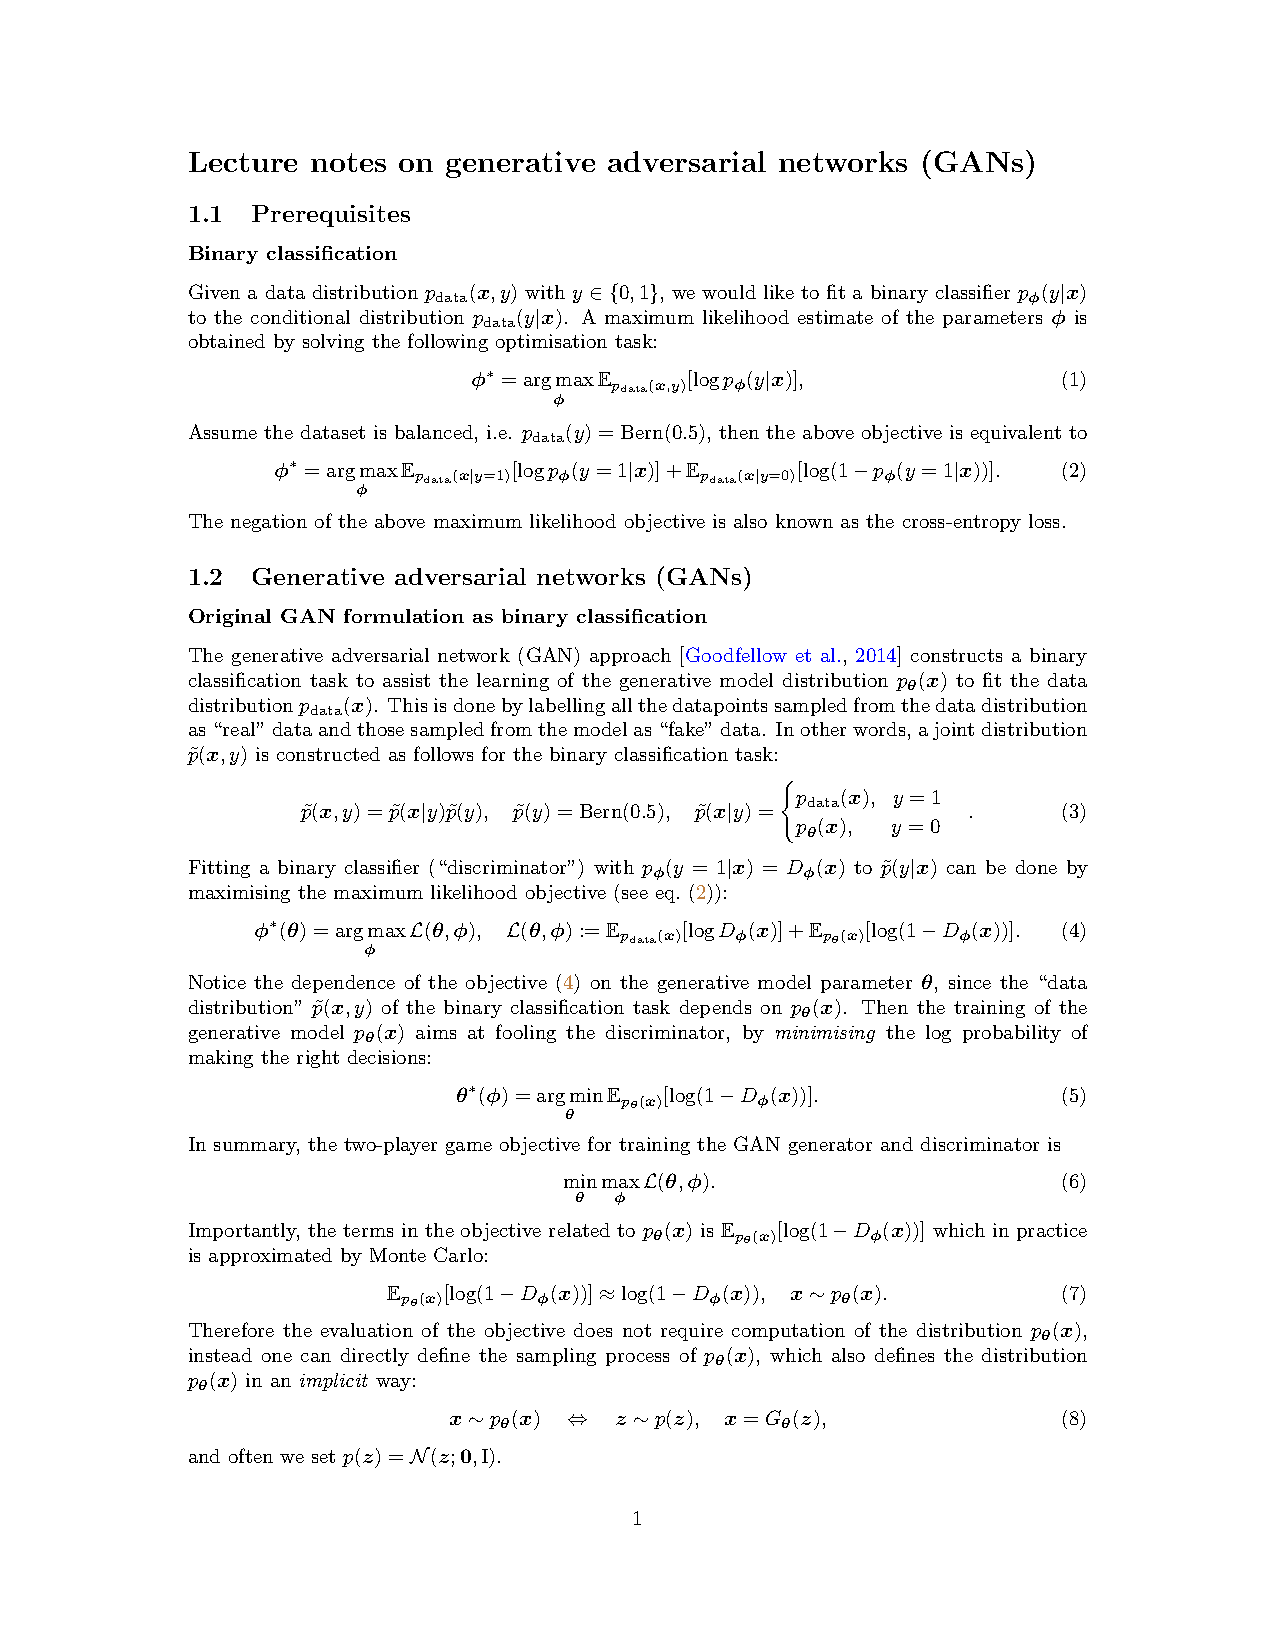
\includegraphics[page=1, trim=2.7cm 3cm 2.7cm 19cm, clip=true, width=\linewidth]{N09_GAN.pdf}}
\end{figure}

The solution of this minmax optimisation task is at equilibrium of the two player adversarial game

\subsubsection{Solution to inner-loop optimisation}

Assuming the discriminator network $D_\phi$ has infinite capacity with fixed $\theta$, we can show that the outermost discriminator is the base classifier, whcih computes the ratio between the data distirbution between and the sum of the data and model distributions.

\begin{equation}
    \phi^* = \max_\phi L(\theta, \phi)\quad \text{satisfies} \quad D_{\phi^*}(x)=\frac{p_{data}(x)}{p_{data}(x)+p_\theta(x)}
\end{equation}

\subsubsection{Equivalence to Jensen-shannon divergence minimisation}

\begin{figure}[H]
    \centering
    \fbox{\includegraphics[page=2, trim=2.7cm 13.8cm 2.7cm 3cm, clip=true, width=\linewidth]{N09_GAN.pdf}}
\end{figure}

This shows that at equilibrium, the generative model is identical to the data distribution, whci justifies the GAN objective as a sensible one to be used for generative modelling.

\subsection{Algorithm}

\subsubsection{Double Loop algorithm}

We need to come up with a convergence theorem fro equilibrium.

\begin{enumerate}
    \item \textbf{Inner Loop}:
    
    With fixed $\theta$, optimise $\phi$ for a few gradient ascent iterations:
    \begin{equation}
        \max_\phi \mathbb E_{p_{data}(x)}[\log D_\phi(x)] + \mathbb E_{p_\theta(x)}[\log(1-D_\phi(x))]
    \end{equation}

    \item \textbf{Outer Loop}:
    
    With fixed $\phi$ from the inner loop, optimise $\theta$ by \textbf{One} gradient descent step:

    \begin{equation}
        \min_\theta \mathbb E_{p_\theta(x)}[\log(1- D_\phi(x))]
    \end{equation}

    \item Loop over (1) and (2) until convergence

\end{enumerate}

In practice, the expectations $\mathbb E_{p_{data}(x)}[\cdot]$ and $\mathbb E_{p_\theta(x)}[\cdot]$ are estimated by minibatches

\begin{gather}
    \mathbb E_{p_{data}(x)}[\log D_\phi(x)] \approx \frac 1 M \sum^M_{m=1} \log D_\phi(x_m), \quad x_m \sim p_{data}(x) \\
    \mathbb E_{p_\theta(x)}[\log(1-D_\phi(x))] \approx \frac 1 K \sum^K_{k=1} \log(1-D_\phi(G_\theta(z_k))), \quad z_k \sim p(z)
\end{gather}

\subsubsection{Pseudo-code}

\begin{figure}[H]
    \centering
    \fbox{\includegraphics[page=40, trim=2cm 2.2cm 2.4cm 4.9cm, clip=true, width=\linewidth]{L07-10_generative_models.pdf}}
\end{figure}

This network is pretty unstable because the two networks are playing an adversarial game. The leraning rate, t, and k parameters matter.

\subsubsection{Initialisation Problem}

Initially, the generator is random, therefore the discirminator can classify with high-accuracy if an image if fake or not: $D_\phi(G_\phi(z))\approx 0$.

\begin{figure}[H]
    \centering
    \subfigure{\includegraphics[page=41, trim=22.35cm 3cm 2.7cm 6.65cm, clip=true, width=.45\linewidth]{L07-10_generative_models.pdf}}
    \subfigure[non-saturated loss]{\includegraphics[page=42, trim=22.35cm 3cm 2.7cm 6.65cm, clip=true, width=.45\linewidth]{L07-10_generative_models.pdf}}
\end{figure}

\begin{itemize}
    \item \textbf{(a)}: In the training procedure, the beining of training, the generator starts from the close-to-zero region. And in this region, the gernerator loss is almost flat, therefore it has very little gradient infromtaiton to help with training.
    \item \textbf{(b)}: Instead, maximise hte porbability of the discriminator to make wrong decsiions on fake data that for theis alternative objective, the graident of the lss with respect to X has a very large norm, which provides a strong learningd signal for a generator to imporve the qluaity of the fake images.
\end{itemize}

\subsection{Wasserstein GAN}

Discriminator can be used to score the provided inputs. The discriminator should asign high scores to data inputs and low scores to fake inputs.

\begin{equation}
    \min_\theta \max_\phi \mathbb E_{p_{data}(x)}[D_\phi(x)]-\mathbb E_{p_\theta(x)}[D_\phi(x)]
\end{equation}

However, this doesn't consider the inifinite capacity of the discriminator network, which should trivially return $D_\phi(x)=_\infty\ if\ x\sim p_{data}(x)\ else\ D_\phi(x)=-\infty$.

\begin{figure}[H]
    \centering
    \fbox{\includegraphics[page=43, trim=21.5cm 2.1cm 2.7cm 12.5cm, clip=true, width=.45\linewidth]{L07-10_generative_models.pdf}}
    \caption*{This results in a very spiky function, and it is constant around the generated images. This has no use for gradient infromation for generator learning.}
\end{figure}

To address this issue we need to make sure that we have useful gradient infromation to learn the generator.

\subsubsection{Using Wasserstein distnace in GANs}\label{app:gan:Using Wasserstein distnace in GANs}

\begin{figure}[H]
    \centering
    \fbox{\includegraphics[page=4, trim=2.7cm 10.6cm 2.7cm 6.3cm, clip=true, width=\linewidth]{N09_GAN.pdf}}
    \caption*{\centering Here, the discriminator should assign high scores to data inputs and low scores to fake inputs. At the same time, discriminator should be smooth to provide useful graident for learning $G_\theta$.}
\end{figure}

\begin{figure}[H]
    \centering
    \fbox{\includegraphics[page=44, trim=2cm 3cm 2.7cm 5cm, clip=true, width=\linewidth]{L07-10_generative_models.pdf}}
    \caption*{To address this problem, we need to make sure that we have useful gradient infromatino to learn the generator. A way to achieve this is to make the discriminator smooth in detail. We firstly, add a contraint that the limshitz-constraint is less than 1, it minimises the wasserstein distance and the supremum is obtained when the discrimintor is one Lipschitz. This creates a stable signal for generating the learning.}
\end{figure}

\begin{figure}[H]
    \centering
    \fbox{\includegraphics[page=45, trim=2cm 1.1cm 1.2cm 5cm, clip=true, width=\linewidth]{L07-10_generative_models.pdf}}
    \caption*{The lipschitz continuity constraint is placed over all possible x inputs, this is intractible. Instead, the WGAN proposed a Lagrange multiplier type of appraoch which minimises the mean suqared error of the difference between the desired and the actual gradient norm}
\end{figure}

$\hat p (x)$ is the auxiliary distribution and is visualised on the rhs figure. First, draw two sets of samples, one for real and fake. Then we run the [UNCLEAR] aginast the real and fake samples and pick in ranodm a point on the line segment connecting the two. 

\section{Advances and Applications}

\subsection{Conditional latent variable models}

The Goal is to learn a generative model $p_\theta(x|y)$

\begin{itemize}
    \item $x$: data to be generated (e.g. an image)
    \item $y$: label/info that the generation process is conditioned on (e.g. fur colour)
\end{itemize}

\subsubsection{Idea 1 | Train a set of models for each feature}

If $y\in \{1, \dots, C\}$ we can train a set of models

\begin{itemize}
    \item $p_\theta(x|y=c)=p_{\theta_c}(x)=\int p_{\theta_c}(x|z)p(z)dz$
    \item Parameter inefficient: need to train C networks
    \item Cannot generalise to continuous $y$
\end{itemize}

\subsubsection{Idea 2 | Make ($z,y$) as the input of the network}

Make both the latent variable $z$ and the conditional variable $y$ as the inputs to the generator network.

\begin{itemize}
    \item $p_\theta(x|y=c)=p_{\theta_c}(x)=\int p_{\theta_c}(x|z,y=c)p(z)dz$
    \item Parameter efficeint
    \item Generalises to continuous $y$
    \item Disentangled the learned representation $z$ from the label info $y$.
\end{itemize}

\subsection{Conditional VAEs}

\begin{figure}[H]
    \centering
    \fbox{\includegraphics[page=50, trim=2cm 1.1cm 1.2cm 5cm, clip=true, width=\linewidth]{L07-10_generative_models.pdf}}
    \caption*{A natural idea is to use maximum likelihood estimation. This, again, is intractible because the conditional distirbution $p(x|y)$ requires integrating out the latent variable $z$. Therefore, we implore the similar strategy for variational lower-bounds.
    
    This is alsmot identical to the original cases, except that now the encoder needs to take in both X and Y as the inputs to produce the distributional parameters $\mu$ and $\sigma$. Similarly, the decoder needs Z and Y as input to generate the reconstruction.}
\end{figure}

\begin{figure}[H]
    \centering
    \fbox{\includegraphics[page=51, trim=2cm 1.1cm 1.2cm 5cm, clip=true, width=\linewidth]{L07-10_generative_models.pdf}}
    \caption*{We can derrive an adverserial training method to train the conditional generative model. In this case we need to modify the task; in the original GAN, we need to distinguish the input images. But now we take in x and label y and assign a label `real or fake' to this input pair.}
\end{figure}

\subsection{Generative Model Architecture Design}

\subsubsection{DCGAN}

\begin{figure}[H]
    \centering
    \fbox{\includegraphics[page=53, trim=2cm 2.7cm 1.8cm 3.3cm, clip=true, width=\linewidth]{L07-10_generative_models.pdf}}
\end{figure}

First reshape the latent variable vector z into a tensor then apply deconvolutions or transposed convolutions to generate the image. The discriminator follows the similar idea, until the final layer which translates the input into a binary classificaiton logit.

\subsubsection{LAPGAN}

\begin{figure}[H]
    \centering
    \fbox{\includegraphics[page=54, trim=2cm 2.7cm 1.8cm 4.8cm, clip=true, width=\linewidth]{L07-10_generative_models.pdf}}
    \caption*{Construct images in a multi-scale fashion. }
\end{figure}

Generating the full image in one shot may be hard. It may be easier to generate small scale versions and scale up. It has a set of generators which generate images at different resolutions. the images are then upscaled into higher resolutions, until the point where the blurry image is given in as a conditional input for the next generator to generate a sharper and refined version of it.

\begin{figure}[H]
    \centering
    \fbox{\includegraphics[page=55, trim=2cm 2.3cm 1.8cm 3.3cm, clip=true, width=\linewidth]{L07-10_generative_models.pdf}}
    \caption*{Training at multiple resolutions}
\end{figure}

To train multiple generators, introduce multiple discriminators at different scales. The idea is that with higher resoultions on a real image it is striaghtforward to downslae it to generate  lower resolution versions. Since upscaling an image is easy, we can produce the difference betwene the original image and the blurred version of it (because the models are incharge of producing refinements).

We repeat this process to train the generator. At the smallest level, we still use the original GAN procedure, however, at this point the iamge resouliton is very low, so the discriminator is less likely to distinguish fake from real | therefore trining may be easier.

\subsubsection{Progressive GAN}

\begin{figure}[H]
    \centering
    \fbox{\includegraphics[page=56, trim=2cm 3cm 1.8cm 4cm, clip=true, width=\linewidth]{L07-10_generative_models.pdf}}
\end{figure}

trains the generator and discriminator networks in a progressive way. Start with a low resolution and train a gan there. After training at that resolution scale, progress up, and train both old and new with higher resolution image. This procedure is repeated.

\subsubsection{StyleGAN}

\begin{figure}[H]
    \centering
    \fbox{\includegraphics[page=57, trim=2cm 2.3cm 1.8cm 4cm, clip=true, width=\linewidth]{L07-10_generative_models.pdf}}
\end{figure}

Idea: the latent variable $z$ represents the concept of stypes of the image. The $z$ varibale is transformed into a style representation vector $w$ which is used at each resolution scale of the generator to normalize and shift the feature mass. The noise contributes to a source of randomness in the image. 

\subsubsection{NVAE | improved VAE image generation}

\begin{figure}[H]
    \centering
    \fbox{\includegraphics[page=59, trim=2cm 3cm 1.8cm 4cm, clip=true, width=\linewidth]{L07-10_generative_models.pdf}}
    \caption*{The paper provides an imporved q distribution to mitigate the challenge of optimisation of the variational lower bound, which tends to prefer smoother image reconstruction.}
\end{figure}

\subsubsection{Combining VAEs and GANs}

\begin{figure}[H]
    \centering
    \fbox{\includegraphics[page=61, trim=2cm 3cm 7cm 4cm, clip=true, width=.8\linewidth]{L07-10_generative_models.pdf}}
\end{figure}

There are recent efforts that try to combine VAEs and GANs | achieve best of both worlds. For VAEs it has an autoencoder architecture which allows us to inferr the latent code Z given an input image. The reconstruction error in VAE, is strong signal for generator training.

\subsubsection{Summary}

\begin{figure}[H]
    \centering
    \fbox{\includegraphics[page=60, trim=2cm 3cm 1.8cm 4cm, clip=true, width=\linewidth]{L07-10_generative_models.pdf}}
    \caption*{GANs tend to produce sharper images}
\end{figure}

GAN is often preffered for better visual quality, VAEs preffered for applications that need good likelihood estimates. 

\subsection{Applications of Generative Models}

\begin{itemize}
    \item Super-resolution
    \item Image-to-image translation | translations between iamges in two domains X and Y
\end{itemize}

\subsection{Other types of generative models}

\begin{itemize}
    \item Normalising flow | translate a gaussian curve
    \item Continuous time generative models
    \item Energy-based models | uses NN to parameterise an energy function - observed data will have low energy, and other points will have high energy.
\end{itemize}



\clearpage

\appendix

\section{Supplied VAE notes}\label{sect:Supplied VAE notes}

\subsection{Prerequisites}

\subsubsection{Probabilistic graphical models}\label{sect:Probabilistic graphical models}

\begin{figure}[H]
    \centering
    \fbox{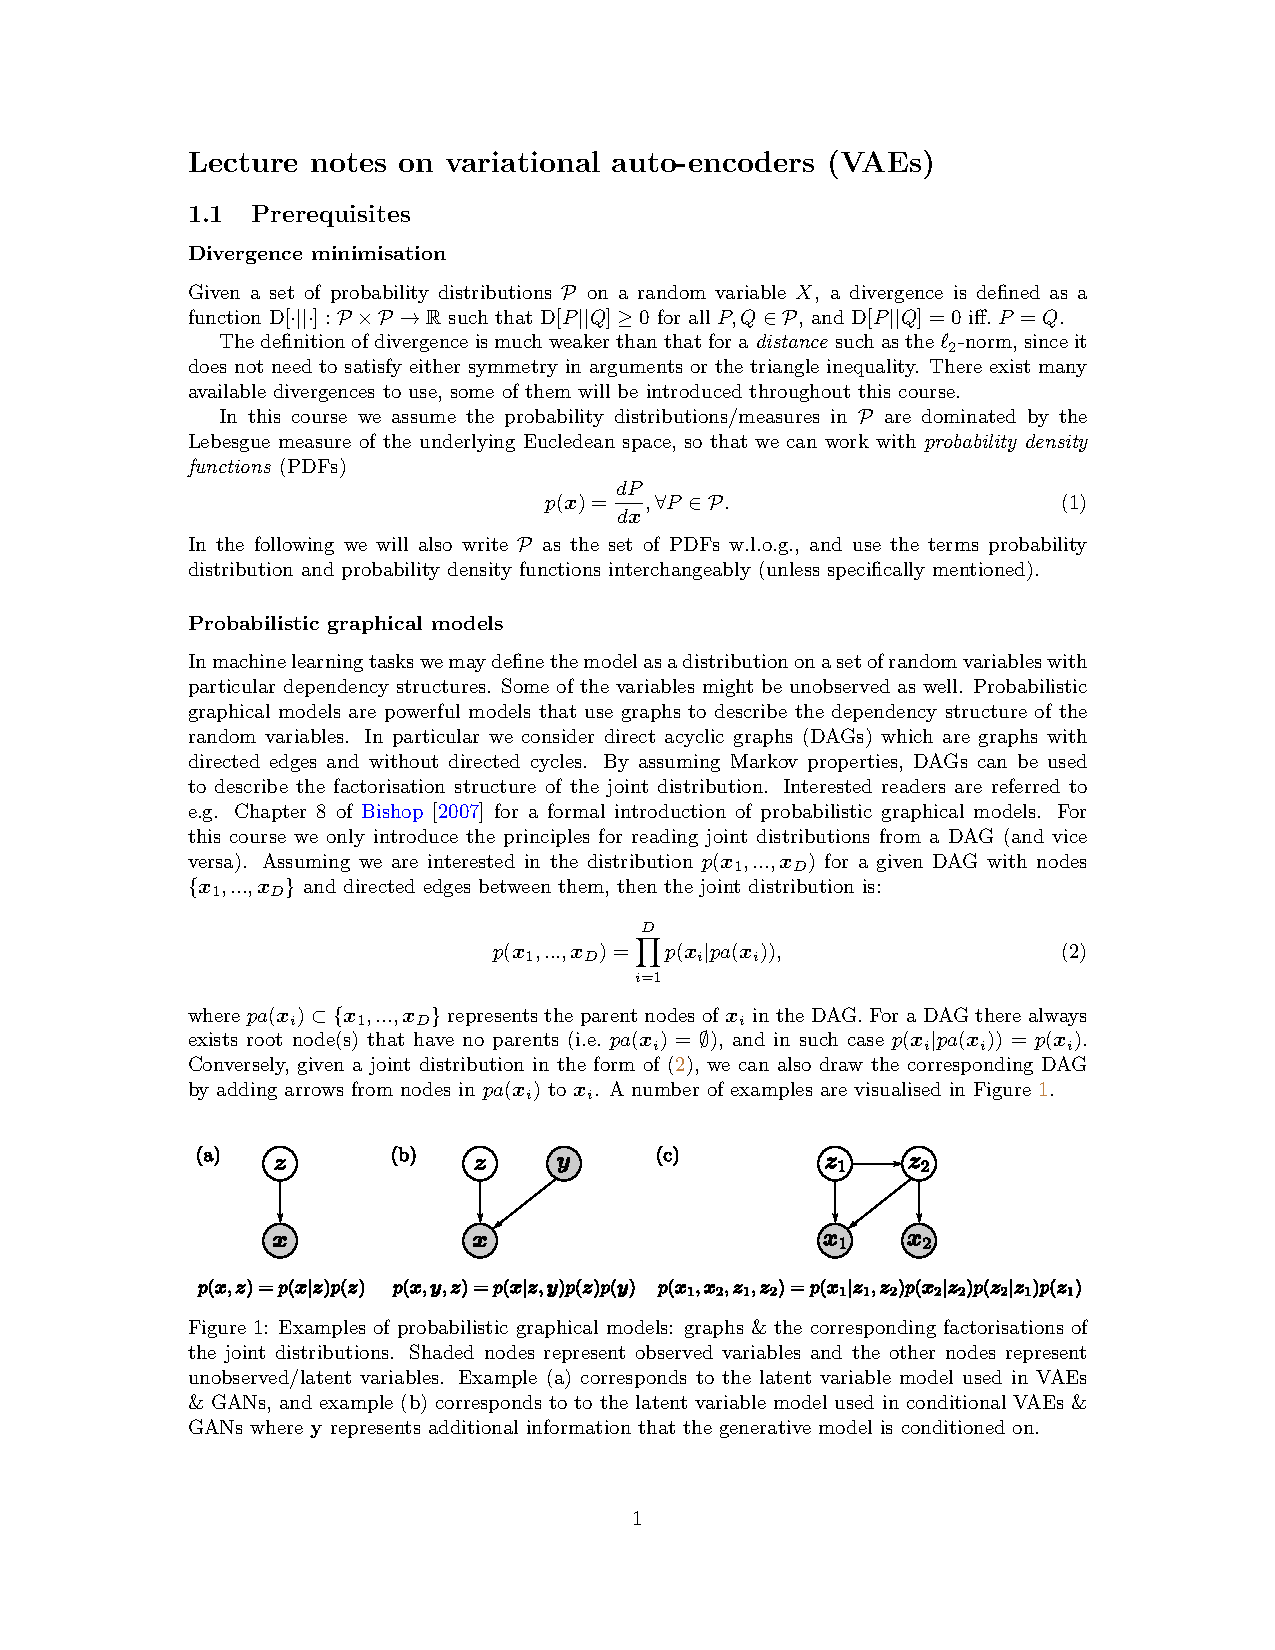
\includegraphics[page=1, trim=2.7cm 3.6cm 2.7cm 11.1cm, clip=true, width=\linewidth]{N08_VAE.pdf}}
\end{figure}

\subsubsection{Jensen's inequality}\label{sect:Jensen's inequality}

\begin{figure}[H]
    \centering
    \fbox{\includegraphics[page=2, trim=2.7cm 8.1cm 2.7cm 3cm, clip=true, width=\linewidth]{N08_VAE.pdf}}
\end{figure}

\subsubsection{Analytic KL between factorised Gaussians}\label{sect:Analytic KL between factorised Gaussians}

\begin{figure}[H]
    \centering
    \fbox{\includegraphics[page=5, trim=2.7cm 14.1cm 2.7cm 2.5cm, clip=true, width=\linewidth]{N08_VAE.pdf}}
\end{figure}

\subsection{Conditional VAE}\label{sect:Conditional VAE}

\begin{figure}[H]
    \centering
    \fbox{\includegraphics[page=6, trim=2.7cm 3.1cm 2.7cm 11.7cm, clip=true, width=\linewidth]{N08_VAE.pdf}}
\end{figure}

\begin{figure}[H]
    \centering
    \fbox{\includegraphics[page=7, trim=2.7cm 19.6cm 2.7cm 2.5cm, clip=true, width=\linewidth]{N08_VAE.pdf}}
\end{figure}

\subsection{\color{red}{*Practical interpretations \& KL annealing}}\label{sect:Practical interpretations and KL annealing}

\subsubsection{Comparisons with auto-encoders}\label{sect:Comparisons with auto-encoders}

\begin{figure}[H]
    \centering
    \fbox{\includegraphics[page=7, trim=2.7cm 11cm 2.7cm 10cm, clip=true, width=\linewidth]{N08_VAE.pdf}}
\end{figure}

\subsubsection{KL annealing}\label{sect:KL annealing}

\begin{figure}[H]
    \centering
    \fbox{\includegraphics[page=7, trim=2.7cm 3.1cm 2.7cm 18cm, clip=true, width=\linewidth]{N08_VAE.pdf}}
\end{figure}

\begin{figure}[H]
    \centering
    \fbox{\includegraphics[page=8, trim=2.7cm 13.5cm 2.7cm 2.5cm, clip=true, width=\linewidth]{N08_VAE.pdf}}
\end{figure}

\section{Supplied GAN notes}

\subsection{Binary Classification}\label{app:gan:Binary Classification}

\begin{figure}[H]
    \centering
    \fbox{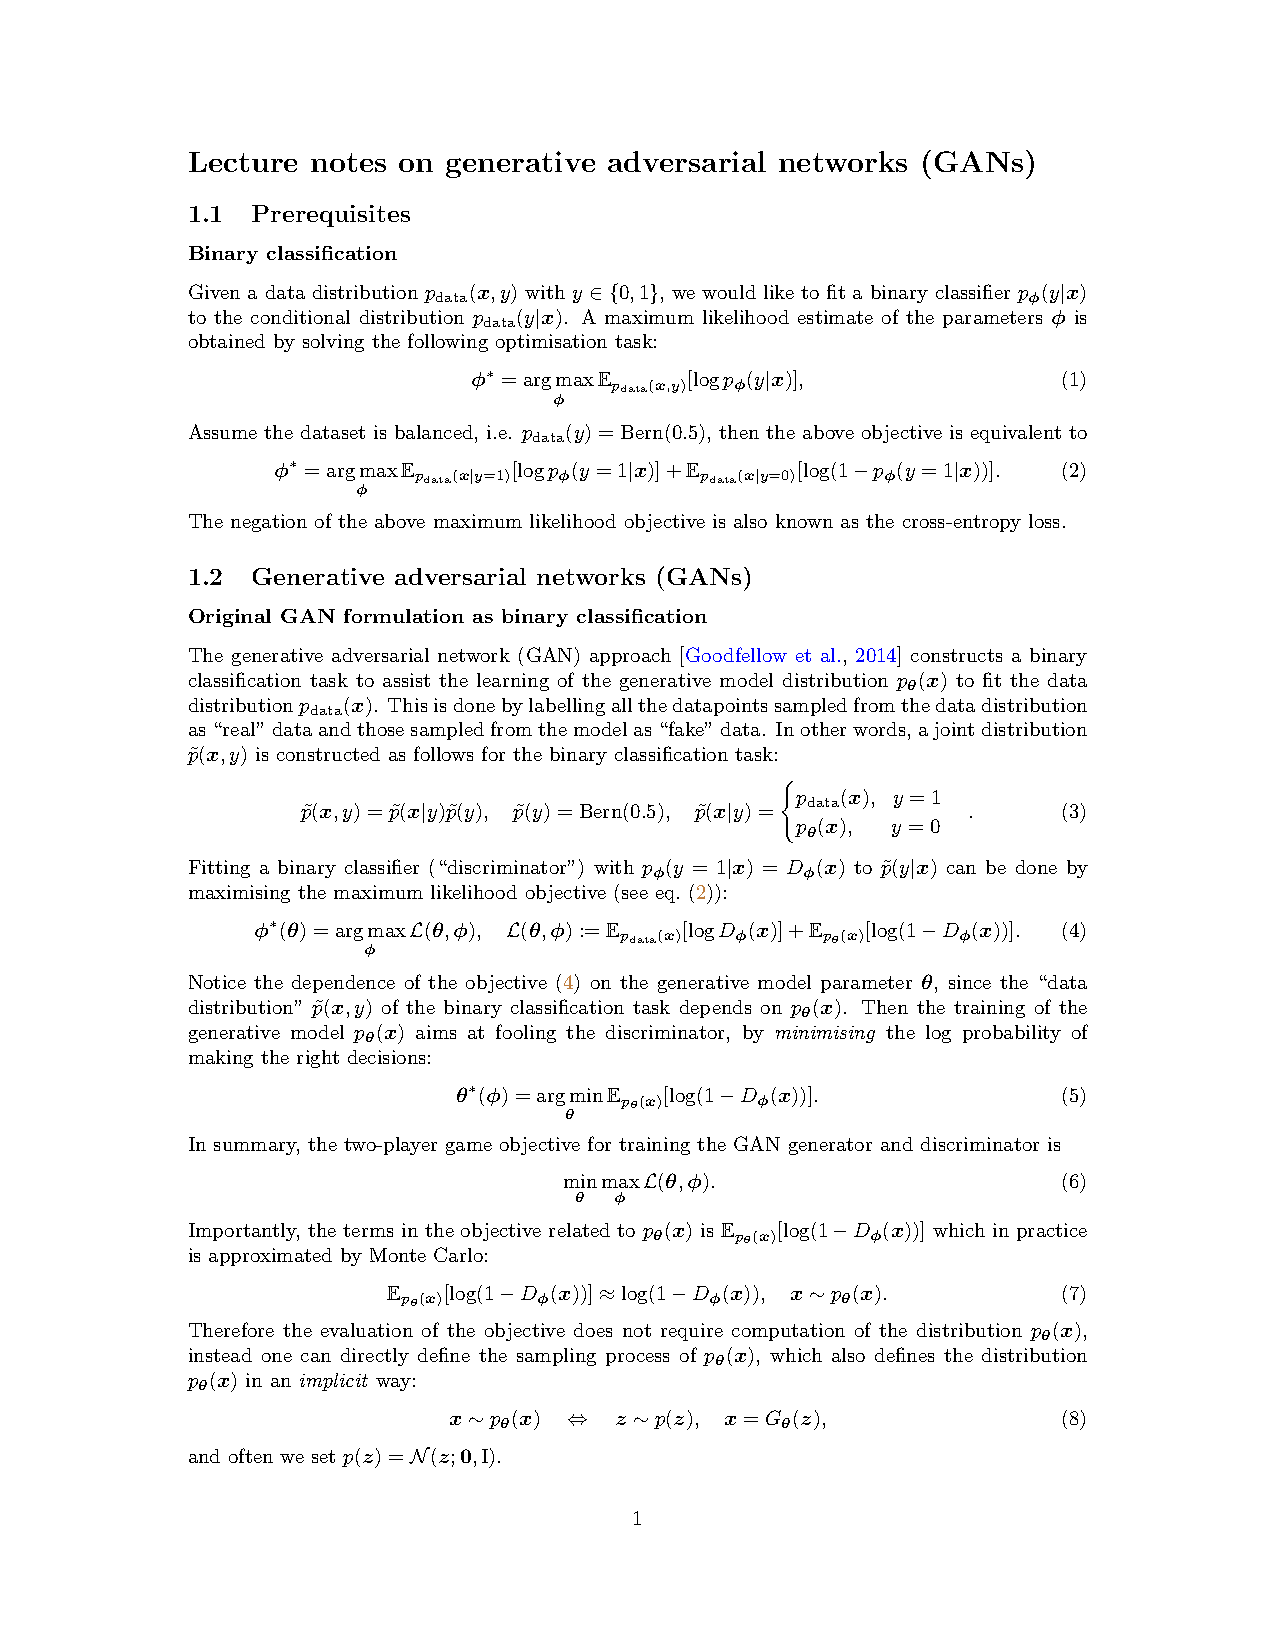
\includegraphics[page=1, trim=2.7cm 18.8cm 2.7cm 4.7cm, clip=true, width=\linewidth]{N09_GAN.pdf}}
\end{figure}

\subsection{Generative adversarial networks (GANs)}\label{app:gan:Generative adversarial networks (GANs)}



% \subsubsection{Equivalence to Jensen-shannon divergence minimisation}

% \begin{figure}[H]
%     \centering
%     \fbox{\includegraphics[page=2, trim=2.7cm 13.8cm 2.7cm 3cm, clip=true, width=\linewidth]{N09_GAN.pdf}}
% \end{figure}

\subsubsection{Alternative loss for the generator}\label{app:gan:Alternative loss for the generator}

\begin{figure}[H]
    \centering
    \fbox{\includegraphics[page=2, trim=2.7cm 3cm 2.7cm 15cm, clip=true, width=\linewidth]{N09_GAN.pdf}}
\end{figure}

\begin{figure}[H]
    \centering
    \fbox{\includegraphics[page=3, trim=2.7cm 19.4cm 2.7cm 2.5cm, clip=true, width=\linewidth]{N09_GAN.pdf}}
\end{figure}

\subsection{Conditional GAN}\label{app:gan:Conditional GAN}

\begin{figure}[H]
    \centering
    \fbox{\includegraphics[page=3, trim=2.7cm 7.5cm 2.7cm 9.6cm, clip=true, width=\linewidth]{N09_GAN.pdf}}
\end{figure}

\subsection{\color{red}{*Wasserstein GAN}}\label{app:gan:*Wasserstein GAN}

\subsubsection{Wassterstein distance}\label{app:gan:Wassterstein distance}

\begin{figure}[H]
    \centering
    \fbox{\includegraphics[page=3, trim=2.7cm 3cm 2.7cm 22.2cm, clip=true, width=\linewidth]{N09_GAN.pdf}}
\end{figure}

\begin{figure}[H]
    \centering
    \fbox{\includegraphics[page=4, trim=2.7cm 22.6cm 2.7cm 2.5cm, clip=true, width=\linewidth]{N09_GAN.pdf}}
\end{figure}

\subsubsection{Integral probability metrics (IPMs)}\label{app:gan:Integral probability metrics (IPMs)}

\begin{figure}[H]
    \centering
    \fbox{\includegraphics[page=4, trim=2.7cm 3.6cm 2.7cm 18.4cm, clip=true, width=\linewidth]{N09_GAN.pdf}}
\end{figure}

\begin{figure}[H]
    \centering
    \fbox{\includegraphics[page=5, trim=2.7cm 16.4cm 2.7cm 2.7cm, clip=true, width=\linewidth]{N09_GAN.pdf}}
\end{figure}

\printbibliography
\addcontentsline{toc}{section}{Bibliography}

\end{document}